% !TEX root = mythesis.tex

%==============================================================================
\chapter{Neutrino Analysis $60^\circ < \theta < 75^\circ$}
\label{sec:DGL}
%==============================================================================
This chapter gives a brief summary of the neutrino search performed for the zenith range $60^\circ < \theta < 75^\circ$. The neutrino search is separated in different angular range to maximise the performance of the detector array in this case the SD for the search. The chapter aims to cover the expected signature in terms of measurable quantities in the Pierre Auger Observatory for the particular angular range, the neutrino simulation used to develop the analysis, the reconstruction chain used along with the quality cuts used for such an analysis. Further, the quality cuts are analysed in more detail especially in the context of improving the capability of the search by the usage of MoPS and ToTd. In the end the improvements to both the diffused and point source neutrino searches with the new triggers are quantified.


\section{SD Neutrino signature $60^{\circ} < \theta < 75^{\circ}$}
\label{sec:sig_DGL}

The strategy and method to detect neutrino showers in this angular range with the SD remains the same as mentioned before i.e to try detecting showers that develop late and have more electromagnetic or "young" shower front at ground. In terms of signal in the SD array the young shower is expected to be spread over a longer time period typically hundreds of nanoseconds and have a lower maximum peak compared to signal induced by older showers which are spread over tens of nanoseconds and have a higher maximum peak. A comparison of the difference between the induced SD signal from a young and old shower arriving from the same zenith angle is presented in fig. ~\ref{}. However, such differences in signals and the ability of the SD to differentiate between a neutrino induced and a proton/ heavy nuclei induced shower disappears for vertical showers($\Theta < 60^{\circ}$). For vertical showers a cosmic ray induced shower does not have enough time to develop because of the limited thickness of the atmosphere. At these zenith angles a high energy CR induced EAS can mimic the expected young shower signature of a neutrino induced EAS at ground. Thus, currently the neutrino searches at the Pierre Auger Observatory are limited to zenith angles above $60^\circ$ where it is much easier to separate a neutrino induced EAS from a CR induced EAS. Since we are also searching for young showers which have not fully developed till they are detected at ground, reconstructed energy cannot be used as a discrimination criterion.      

To select the longer signals in the SD one of the variables that was used in erstwhile neutrino searches is the fraction of ToT-T2 triggered signals in the recorded event. As mentioned in the previous chapter this trigger is tuned to select broader signals which for an inclined shower is evidence of a young shower. For the search presented in this thesis along with the ToT-T2, the ToTd and MoPS are also used. Both ToTd and MoPS as mentioned in sec.~\ref{} help further increase the selection efficiency for broader signals by reducing the impact of low energy muons. These muons which form the majority of the background at low zenith angles of the selected search range. Thus, these triggers are impactful in increasing the separation power for low energy($\leq$ 1 EeV) neutrino showers. Another important variable which is used to judge the width of the signals is Area Over Peak (AoP). The AoP is defined as the ratio of the integrated signal of the station over the biggest value or peak of the signal. The AoP is calibrated in such a way that narrow/ old shower signals have AoP ~ 1 while broad/old shower signals have AoP $\geqslant $ 1. 



\section{Neutrino Simulations}
\label{sec:sim_DGL}
To characterise the neutrino search ability of the Pierre Auger Observatory Monte Carlo simulations of EASs induced by UHE$\nu$s are required. There are six possible neutrino interaction chanels due to the three possible neutrino flavors with each having two possible channels(CC or NC). However, for simulations these are envisioned to be characterised by just two sets of simulations. For the NC channel since the EAS induced by three neutrino flavors has the exact same signature for our detector only $\nu_e$ NC simulations were performed to estimate the NC contribution of all the three flavors to the final exposure. 

For the CC interactions in the case of $\nu_{\mu}$ the resulting high energy muon has a high probability of evading detection. This is very similar to the NC interaction where the resultant secondary neutrino also carries approximately 80\% of the primary energy. Thus, after taking into account the appropriate crossection, in principle the NC simulations can be used to also estimate the contribution of $\nu_{\mu}$ CC channel.  

In the case of $\nu_{\tau}$ CC interactions where the resulting $\tau$ especially at higher energies($\geq $EeV) can decay and also initiate a secondary shower resulting in a "double bang" like signature in the Observatory. In the context of this thesis such signatures are not accounted for and the $\nu_{\tau}$ CC interaction is treated in the same way as the $\nu_{\mu}$ CC interaction resulting in a possible underestimation of the Observatory to $\nu_{\tau}$ events. A future $\nu_{\tau}$ simulation library is currently being prepared by the Pierre Auger Collaboration Monte Carlo task and could help extend this analysis in the future.

Thus, in summary $\nu_e$ CC and NC simulations can be considered to be good approximations to estimate the contributions of all the other channels to the overall exposure of the Observatory. The simulations were produced in two parts by the Pierre Auger Collaboration Monte Carlo task based on the GAP note ~\ref{}. The first part entails the simulation of the $\nu$ induced EAS in the atmosphere and the second consists of simulating the appropriate detector response for the corresponding shower. 

\subsection{Atmospheric Shower simulations}
\label{subsec:sim_EAS}
The first part included using CORSIKA~\ref{} to generate the EAS initiated by a $\nu$ primary. This involves simulating the primary neutrino-nucleon interaction which is performed in CORSIKA using the HERWIG code. Further options such as CHARM to track charm secondaries are not used. Also since only $\nu_e$ simulations are simulated, the TAULEP option which handles $\nu_{\tau}$ and $\overline{\nu_{\tau}}$ is also not used. The systematic uncertainties related to the primary interaction estimator is discussed later in section~\ref{}. CORSIKA further tracks the primary interaction products as they travel in the atmosphere towards the ground constituting the air shower. CORSIKA offers a wide variety of choice regarding selecting the hadronic interaction model. For the simulations used in this study separate high and low energy hadronic interaction models were used. For energies higher than 200 GeV three high energy hadronic models QGSJETT~\cite{}, SYBILL~\cite{} and EPOS-LHC~\cite{} were compared. The results of the comparison are mentioned in detail in Appendix~\ref{}. Since the differences between the models are not that significant for the neutrino analysis ....dash..... was chosen as the high energy interaction model. For lower energies FLUKA~\cite{} was chosen. The systematic uncertainities arising from different models are discussed in section~\ref{}.  

To account for the curvature of the Earth which is especially important for the zenith angles studied, the EGS4~\ref{} Monte-Carlo method is chosen to simulate the electromagnetic component of the shower. The analytical NKG~\ref{} method which is also available but is not used for these simulations since it vastly underestimates the maximum of the electromagnetic component due to the fact it does not account for a curved atmosphere. GDAS Malargue October atmospheric profile is chosen for the simulations and the magnetic field components are taken to be the default values at the Malargue site ($B_x = 19.52\mu T$ and $B_z = -14.17\mu T$). 

Further, since the computing times taken for shower simulations scale roughly with the primary energy, for primary energies > $10^{16}$eV these times become extremely long. Though parallel computing provides a viable solution, the technique of "thin sampling" or thinning~\cite{} offers an alternate way to reduce the computation times while simultaneously saving wastage of resources. The thinning algorithm is applied to all particles below the adjustable fraction of the primary energy which emerge from an interaction. Only one of these particles is followed ,and a proper weight is assigned to this particle to account for the untracked ones which are dropped based on the thinning level($\epsilon_{th} = E/E_0$). Additional improvements ~\cite{} which reduce the statistical fluctuation of particle densities far from the shower core using a maximum limitation of weights and reduction of number of particles close to the shower core where the detectors anyway have a high chance of saturation are also used as a part of thinning algorithm in CORSIKA. A thinning value of $10{-6}$ is used for the simulations in this study. An example of the CORSIKA input file used by the MC task to produce the simulated showers is shown below:

\todo{Add The CORSIKA steer file}

The simulations were performed using the GRID technology~\cite{}. Both CC and NC showers were simulated for fixed energy steps of log(E/eV) = 0.5 in the range $10^{17}-10^{20.5}$eV. The number of simulated showers was varied depending on the Energy, atmospheric depth of interaction and the injected zenith angle. More showers were simulated at lower energies and the energy dependent numbers are tabulated in table~\ref{}. Further, for both the interaction channels within the zenith angle range $60^{\circ}-70^{\circ}$ the neutrinos were forced to interact at fixed atmospheric depths in steps of 100 g cm$^{-2}$. The injection points both close to the ground where a neutrino shower might have a lower trigger efficiency and close to the top of the atmosphere where a neutrino induced shower might mimic one induced by a proton are rejected for the simulations. The azimuthal angle is left free and can take any value between 0$^{\circ}$ and 360$^{\circ}$. The simulated depths for each zenith angle bin are summarised in table~\ref{}. 

Based on (E,$\theta_{MC}$,X) bin the number of CORSIKA showers simulated vary. Higher values were chosen for lower energies to increase the statistics since at these energies the simulated shower has a higher chance of not being detected be the detector.  

After the simulation is completed CORSIKA produces a normal particle output file which contains information about the surviving particles on the ground level which is set based on the detector elevation. The file contains the relevant information such as energy, momentum, timing all segregated for each particle based on its Particle Data Group Code~\cite{}. It also produces a ".long" file which contains longitudinal distribution of various particle numbers along with the energy deposited which is relevant for fluorescence telescope based analyses. For this work the normal particle output files were used for further processing to simulate a response in the Pierre Auger Observatory SD.

\subsection{Surface Detector Response}
\label{subsec:sim_SD_resp}

The next step required to complete the $\nu$-induced shower simulation is to generate an appropriate detector response in the SD array for each simulated atmospheric shower. This is done using the Offline framework. The framework can read in the CORSIKA output files, undo the applied thinning, simulate the Cherenkov light which will be produced as the particles travel through the WCDs and then also mimic the corresponding WCD electronics outputting the trigger and event information for each simulated shower akin to how real showers are measured at the Observatory. Each step is performed using special modules. The module sequence used to simulate the detector response for $\nu$-induced showers in this thesis is given below: 

\todo{Add The module sequence}


The \textit{EventFileReaderOG} reads in the CORSIKA output file. The following steps are performed assuming an "ideal" SD array with every station operational and fully efficient within the design limts. The steps are also repeated for an individual shower between 5- 30 times depending on the primary energy to further increase the statistics for each (E,$\theta$,X) bin. The first module is the EventGeneratorOG sets the core position, time and event ID for Monte Carlo events. In this analysis similar to ~\cite{} the core position is only allowed to be randomised over a 5 x 5 km$^2$ area around a fixed station at the center of the array. This allows an in depth study of how core position could impact the reconstruction which is discussed later. In the next step the \textit{CachedShowerRegeneratorOG} reads in the list of the shower particles and unthins each particle injecting a set of new particles based on its unique weight~\cite{}. It can then create a list of particles for each SD station which is then passed to the next module \textit{G4TankSimulatorOG}. G4TankSimulatorOG uses Geant4~\cite{} to simulate the particle trajectories in the WCD and the corresponding Cherenkov light produced by these particles. It also handles all the possible absorption and reflection the light can suffer before it is measured by the PMT. Following this the \textit{} simulates the detector calibration constants described in section~\ref{} and the \textit{SdPMTSimulatorOG} takes in the information from the tank simulator and simulates a corresponding PMT signal(trace). \textit{SdFilterFADCSimulatorMTU} and \textit{SdBaselineSimulatorOG} further simulate the processing of the PMT signal by the electronics at each station with the first applying the filter response and the FADC sampling and the second adding baseline and simulated noise to these traces. 

The next two modules decide whether the simulated event fulfills the heirarichal trigger system of the Observatory explained in section~\ref{}. \textit{TankTriggerSimulatorOG} checks if the signal fulfills the local station criteria i.e T1 and T2 condition after which the \textit{CentralTriggerSimulatorXb} further combines all the station which fulfil the T2 criteria to form the T3 simulating the task performed by CDAS for real data. The \textit{CentralTriggerEventBuilderOG} and \textit{EventBuilderOG} then facilitate the transfer of events passing the T3 criteria from the simulation container class to the event class with the last module \textit{EventFileExporterOG} responsible for exporting all the processed showers now with the applied detector response in a file which can be further used for further reconstruction.  


\section{Shower Reconstruction}
\label{sec:reco}

The event reconstruction is a necessary step before any further analysis can be performed. This procedure is developed first for neutrino simulations to enhance their identification efficiency and then applied to real measured data for both estimating the possible background for a neutrino like events and for the final search for neutrinos at the Observatory. Shower reconstruction is also performed within the Offline framework with a module sequence that contains a combination of some standard reconstruction modules and some specific modules developed for neutrino identification in GAP note~\cite{}. The reconstruction is again performed with the help of the MC task on the GRID framework based on the particular reconstruction chain developed for neutrinos. The Module sequence used to reconstruct simulated neutrino showers is given below:

\todo{Reco modulesequence}

The sequence remains similar to the one used in~\cite{} apart from the iterative development performed by the Offline developers over the years. For data reconstruction the \textit{SdMonteCarloEventSelectorOG} is omitted from the sequence. The chain can be subdivided to three main parts which are "event reading and pre-selection," "angular reconstruction" and "posterior selection and export" which are discussed in the next few sections.

\subsection{Event reading and pre-selection}
\label{subsec:reco_presel}

The first module in this part of the reconstruction is again the \textit{EventFileReaderOG} which depending on the input format can parse the file. In the reconstruction sequence it is used to read in either the detector response simulated file for simulations or the measurement files obtained from the SD. The \textit{EventCheckerOG} further checks if the stations in each read event have proper timing information. After this point the FADC traces are processed with various modules to covert them to VEM units. The \textit{SdGainRatioCorrectorKG} corrects for the gain ratio for the electronics followed by \textit{TriggerTimeCorrection} which further corrects for differences in electronics especially related to timing for data over the course of its operation. The \textit{SdStationCheckerOG} further checks the station quality and appropriately sets silent stations if they do not contribute to the final trigger formation. After this point the \textit{SdHistogramFitterKG}, \textit{SdBaselineFinderKG} and \textit{SdTraceCalibratorOG} which get the calibration constants from the calibration traces, fit the baseline and the convert the traces to VEM units respectively. Further modules \textit{SdStationPositionCorrection} corrects the positional differences that might arise due to faulty GPSs which is important for correct timing information, \textit{SdBadStationRejectorKG} sets known bad stations in the array to be inoperational and the \textit{SdSignalRecoveryKLT} which tries to recover signals from the saturated PMTs if any by looking at the undershoot value~\cite{}. An extra module \textit{SdPMTQualityCheckerKG} is also used in the case of data reconstruction to estimate the quality of the detector.

The next three modules are used to fine tune the selection of signals and later events to improve the both the quality of simulated and measured data to increase the efficiency of neutrino detection. The first one is the \textit{SdEventSelectorOG} which applies a basic SD event selection which is also used in other analyses. The module sets conditions based on T4, T5 and other station based parameters if appropriate. The different operations performed by the module are as follows:

\begin{description}
  \item $\bullet$~\textbf{Bottom-up Selection:} This selection helps in deciding the non-participating stations if the stations are not compatible with a planar shower front propagating at the speed of light hypothesis~\cite{}. Such stations can arise due to random noise in the array or due to random coincidences between non-air shower events with air shower events. The selection requires a minimum of three stations which fit the planar front of the shower within lenient time tolerances. It also removes isolated stations by checking the distances to nearest neighbors. Though, the selection is applied, it is not very effective for inclined showers(>$60^{\circ}$) since the showers above these angles are not geometrically compact. Thus, this selection is supplemented with an extra top-down selection implemented in \textit{SdTopDownSignalSelectorUGR} which is discussed later. 
  \item $\bullet$~\textbf{T4 and T5 trigger:} The module also calculates the T4 and T5 criteria discussed in sec.~\ref{}. It also then further discards events if they do not fulfill these criteria. In this study the T4 criteria was not required but a stringent 6T5 criteria was required for the selection. 
  \item $\bullet$~\textbf{Lightning Rejection:} The lightning events can be detected in the SD stations by looking for oscillatory signal in the FADC trace of all three PMTs~\cite{}. For this analysis if any lightning like signal is detected in any one of the stations the whole event is rejected from the analysis. 
  \item $\bullet$~\textbf{ToTd and MoPs trigger:} The module can also silence particular triggers before applying the selection. This feature is used to produce two sets of reconstruction files one with the triggers turned off and one with them turned on. This can impact the number of events fulfilling the 6T5 conditions and thus the overall number of events which can be seen later.    
\end{description}

The \textit{MonteCarloEventSelectorOG} further removes stations with distance in shower plane coordinates smaller than the inner radius used in the CORSIKA simulations. It also removes dense stations i.e virtual stations which are sometimes used for MC studies since these are not representative of the regular SD array. 

The \textit{SdTopDownSignalSelectorUGR} is a module developed specially to carry out a top-down selection and accidental signal rejection for neutrino like events. A summarised overview of what this module aims to accomplish is given next with a detailed description of the module already published in ~\cite{}. The Top-down procedure is applicable for both the simulations and measured data whereas the accidental signal treatment is only applied for measure data. The procedure is based on~\cite{} and ~\cite{}. Top-down selection requires a minimal of three station with the shower front time tolerance compatibility dependent on the zenith angle. If the fit does not converge stations are successively removed and re-tested until a satisfactory fit is achieved. At the end of the procedure stations which do not contribute to the final fit are rejected while the others are marked as candidate stations. Further the Top-Down procedure also takes into account the individual traces and uses the shape for 3-fold topologies. It also rejects isolated signals akin to the Bottom-up selection but with larger tolerances to account for the wider footprint of inclined events. The module also applies an accidental signal rejection procedure before the top-down procedure is applied to account for the atmospheric muon background. The atmospheric muons and also local showers can either trigger isolated stations or even real event stations affecting the start times and in turn the zenith angle reconstruction. This miss-reconstruction can either cause problems with the fitting of the top-down procedure and can also lead non-neutrino like or background events pass the analysis cuts affecting the overall neutrino detection efficiency. The module discards stations with total signals below 3 VEM which rejects the muonic background which typically peaks at 1 VEM. The discarding procedure is implemented only till the minimal number of stations present in the event are below 6. 


\subsection{Angular Reconstruction}
\label{subsec:reco_presel}

The angular reconstruction forms the basis for neutrino detection using the SD especially since for inclined neutrinos the energy reconstruction algorithms typically used for cosmic rays at the Pierre Auger Observatory become unreliable. The angular reconstruction is performed by the \textit{SdPlaneFitOG} and \textit{LDFFinderKG}. The energy reconstruction using the SD is either typically done using the \textit{LDFFinderKG} which fits a lateral distribution function to the SD signal based on the NKG approximation. The NKG approximation is typically inaccurate for inclined showers above a zenith of $60^{\circ}$ thus alternate methods based on muon maps are used for inclined showers. These also fail for neutrino induced showers usually having a large electromagnetic component. Thus, without a reliable energy reconstruction angular reconstruction becomes vital for neutrino induced shower detection at the SD. 

The angular reconstruction procedure uses the timing information from the stations to fit either a plane or a spherical shower front. The axis of shower $a$ is initially assumed to intersect the ground at some time using a signal weighted barycenter $x_b$ and bary-time $t_b$ of selected stations located at $x_i$ with start time $t_i$ given by :




The choice of the weights taken as $\sqrt{S} $ with $S$ being the signal of the stations has been previously evaluated using Monte-Carlo studies~\cite{} to give the best results. The barycenter also serves as the first estimate of impact position of \textit{shower core} at ground but is later estimated more accurately. The shower core is assumed to be moving in the $-a$ direction. Under the plane-front assumption the particles in the shower front move in a plane perpendicular to the shower axis($shower plane$) with the same speed as the core of the shower which is the speed of light c, the time t(x) when the shower plane passes through some chosen point
x (e.g. a station on the ground) can be inferred through a simple projection onto the shower axis as,


Assuming a minimal change in altitude which is true for SD location and precise knowledge of station locations the deviations in estimating the geometrical shower parameters can be due to the uncertainity of the observed start times $\sigma_t$. Thus, the following function needs to be minimised to fit the model for the measured signal start times 


The start time variance needs to be modified for the new triggers and has been taken from~\cite{}. Replacing the axis with $a =(u,v,w)$ and the station coordinates with $x = (x,y)$ (ignoring altitude z). Adding the constraint $u^2 + v^2 + w^2 = 1$ the $chi^2$ can be easily solved. The solution only fails if the stations used while fitting have a linear dependence(three stations in a line) but for higher station multiplicity this is highly improbable especially for the theta range explored for the DGL channel. For more inclined events different solutions to the zenith estimation are used~\cite{}. 
 
Another shower front estimation technique based on a curved shower front approximation is also used to fit the measured stations~\cite{}. The reconstruction assumes the shower development starting at time $t_o$ from a point of origin $x_o$ propagating toward the ground as a concentrically expanding sphere with the speed of light, $c$. The arrival time can thus be estimated as:


As can be seen by the equation, the spherical fit is decoupled from any prior knowledge of the shower core or the shower axis. It is only dependent on the point of origin. Quantities such as shower axis can be determined later when the impact point has been estimated as $x_o -x_c/ x_o-x_c$. The expected solid angle differences between the two fits are of the order of half a degree. The curvature shower front fit is only used for station multiplicities greater than five. This is so because for lower station multiplicities the degrees of freedom are not enough to solve for the shower-front curvature(R-$\infty$). 


\subsection{Posterior selection and Export}
\label{subsec:reco_possel}

The last part of the shower reconstruction chain includes the application of the \textit{SdEventPosteriorSelectorOG} module which computes the 6T5 \textit{posterior} trigger differing from the 6T5 criteria mentioned earlier. The 6T5 posterior requires the 6 stations in the first crown from the nearest station to the reconstructed shower axis to be active or alive during the event. The events which do not pass this criterion are rejected. The last module \textit{RecDataWriterNG} exports all the relevant information to ADST~\cite{} files. In case of reconstructed simulations both the simulated and reconstructed information is stored while for measured data only the reconstructed information is stored.


\section{Reconstructed $\nu$ simulations}
\label{sec:reco_possel}
This section includes some sanity check to check and verify the quality of the $\nu$ simulations. Fig shows the  Efficiency of the reconstructed showers as a function of the zenith angle and the slant depth. The next figure shows the frequency of reconstructed events based on the core position. The non-uniform distribution with the minimal events for core positions close to the stations can be explained due to two reasons. The first being the removal of stations if the PMTs for the particular station is saturated. This saturation can occur for stations very close to the core. The second reason  



\section{$\nu$ selection}
\label{sec:nu_sel}
This section tries to describe the decisions made to select $\nu$ induced air showers. The selection is optimised and evaluated on the above-mentioned neutrino simulations and a part of measured data used as an estimate for the expected background. Since a \textit{blind search} strategy is envisioned for the search. The rest of the measured data forms the \textit{search sample} and will be used to look for neutrino like events during \textit{unblinding}. 
In the first part the selection used to select $\nu$ showers is described in more details. The selection consists of some pre-selection cuts applied to enhance the reconstruction quality of the selected events followed by a Fisher Linear Discriminant~\cite{} based on experimental observables which is the main criteria of differentiation between a $\nu$ induced air shower and background.  
In the second part the performance of the selection is further evaluated based on temporal changes such as aging in the surface detector along and the neutrino detection efficiency is quantified. Comparison to previously used selection are also discussed especially in the context of the performance improvements achieved by using new triggers for neutrino detection.

\subsection{Samples Used}
\label{subsec:nu_sel_samp}



\begin{figure}[t!]
\centering
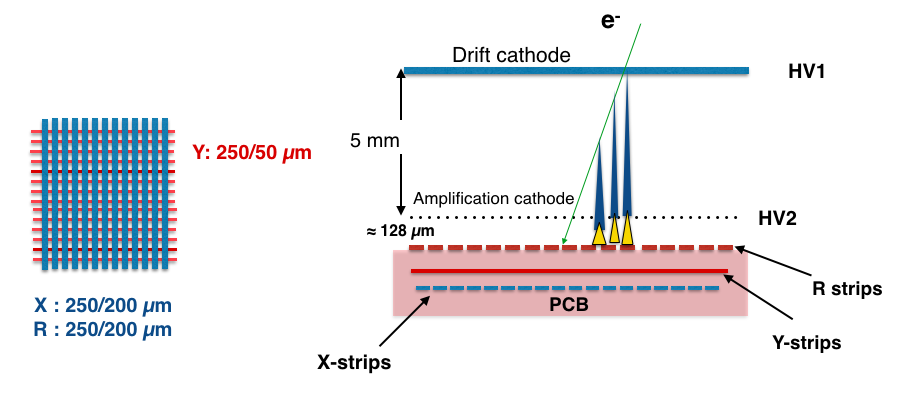
\includegraphics[width=\textwidth]{thesis_figures/NA64_MM.png}
\caption{Left: Strip dimensions of the modules, Right:NA64 Micromega's working principle~\cite{Banerjee:2017mdu}}
\label{fig:Micromegas_na64}
\end{figure}

\subsection{Gas Electron Multiplier}
\label{sec:GEM}

 \begin{figure}[t!]
 \centering
   \begin{minipage}[t]{.45\textwidth}
     \centering
     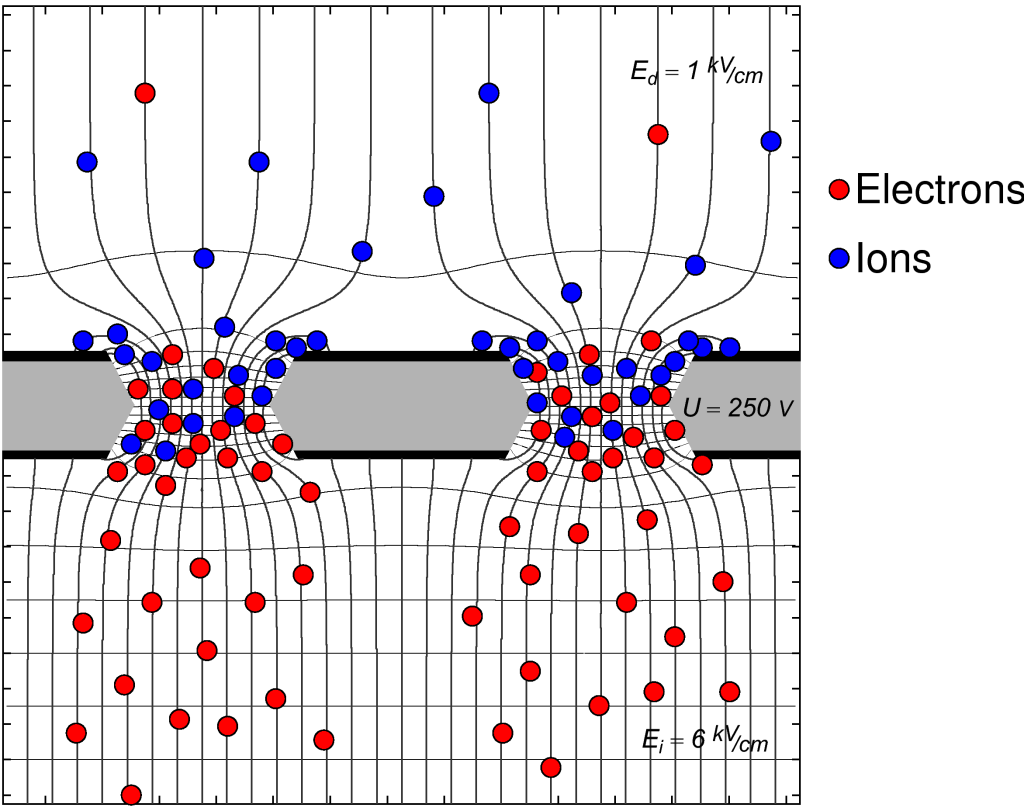
\includegraphics[width=\linewidth]{thesis_figures/GEM_field.png}

     \caption{A sketch of GEM field lines~\cite{GEM_field}.}
     \label{fig:GEM_field}
   \end{minipage}
   \hfill
   \begin{minipage}[t]{.45\textwidth}
     \centering
     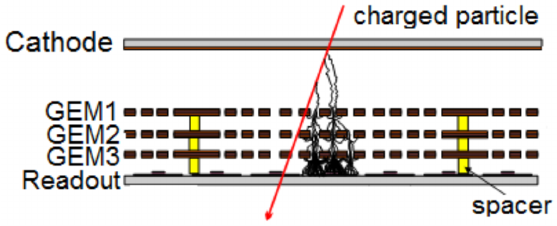
\includegraphics[width=\linewidth]{thesis_figures/GEM_process.png}
     \caption{Schematic of a triple GEM detector along with the working principle~\cite{article_GEM_pic}}
     \label{fig:Triple_GEM}
   \end{minipage}
 \end{figure}

\section{Track-Reconstruction Algorithm}

\subsection{Linear Regression}
\label{sec:Linear_Regression}
Linear regression for track fitting involves fitting a straight line to the data points, hits in our case with the condition that the total error is minimized. The total uncertainty is calculated as a sum of squares of individual measurement errors. Since the final result is dependent on minimizing the sum of the squares this approach to linear regression is known as least-squares approach. A simple mathematical description of the method is given below.

The equation of a straight line is given by $y=mx + c$, where $m$ is the slope of the line and $c$ is the intercept on the $y$ axis in a Cartesian coordinate system. The final goal is to obtain a good estimate for the two parameters $m$ and $c$. To obtain this estimate the square of error needs to be minimized. The error is the difference between the actual measurement $(x_i,y_i)$ and the prediction from our model, the equation of straight line. This error is also known as the residual and is defined as $r_i = y_i - m x_i - c $ for an $i^{th}$ measurement. Suppose that $n$ hits are measured then to obtain an estimate for $m$ and $c$ we need to minimize $\sum_{i=1}^n r_i^2$. The minimized estimates have the following values:
\begin{equation}
      \text{min}(m) = \frac{\sum_{i=1}^n x_i y-i - 1/n \sum_{i=1}^n x_i \sum_{i=1}^n y-i}{\sum_{i=1}^n x_i^2 - 1/n ()\sum_{i=1}^n x_i)^2}  = \frac{\bar{xy} - \bar{x}\bar{y}}{\bar{x^2-\bar{x}^2}}
\end{equation}
\begin{equation}
      \text{min}(c) = \bar{y} - \text{min}(m) \bar{x}
\end{equation}

A more detailed mathematical description can be found in \cite{Linear_regression}. The quality of the fit can be evaluated by calculating the reduced chi-square $\chi^2_{red}=\frac{\chi^2}{ndf.}=\frac{1}{ndf.}\sum_i \frac{(r_i)^2}{\sigma^2}$ where $\sigma$ is the resolution of each detector which might not be equal and ndf. are the number of degrees of freedom available for the fit.

Linear regression can also be used for NA64 to fit for the bending due to the magnets by replacing the model function from the equation of the straight line to some polynomial function. Such a method is called polynomial regression~\cite{STIGLER1974431}.

\begin{figure}[t!]
\centering
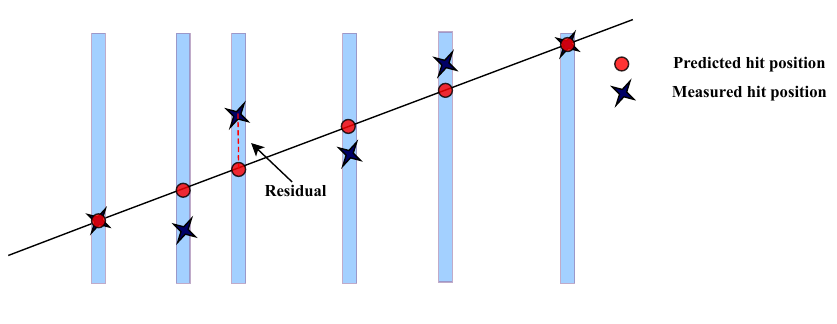
\includegraphics[width=\textwidth]{thesis_figures/linear_reg_new.png}
\caption{Linear regression pictorially. }
\label{fig:linear_regression}
\end{figure}

\begin{description}
  \item $\bullet$~\textbf{Filtering} is estimating the "present" state vector taking into account all the present and "past" measurements. Filtering from $m_1$ to $m_k$ includes filtering $m_1$ to $m_{k-1}$, then propagating from $m_{k-1}$ to $m_k$ and including $m_k$.
  \item $\bullet$~\textbf{Prediction} is estimating the state vector at a "future" time.
  \item $\bullet$~\textbf{Smoothing} is estimating the state vector at any point based on all the measurements.
\end{description}



%%% Local Variables:
%%% mode: latex
%%% TeX-master: "mythesis"
%%% End:
